\section{Infrastructure}
This section will discuss the current backend and frontend services and how they are put together. Each section will have a diagram depicting the system that creates the OMS website, comprised of the services involved and their interactions with each other. Arrows in each section depict the flow of content and information.

\subsection{Current Infrastructure}
Our current infrastructure uses GoDaddy as an End-To-End (E2E) solution. An E2E system has a solution for every part of the process of a deployment pipeline. For us, GoDaddy accommodates the entire website publishing spectrum, beginning from the writing and drafting, to publishing and design, and concluding at the eyes of the audience. Every service is consolidated under GoDaddy making it a one-stop-shop for everything, begetting convenience for simple content management.

I suppose E2E infrastructure was implemented because the GoDaddy route at the inception of OMS (previously On Century Avenue), was a conventionally tried-and-true, albeit severely sub-par, method of website creation.

\begin{figure}[h]
    \centering
    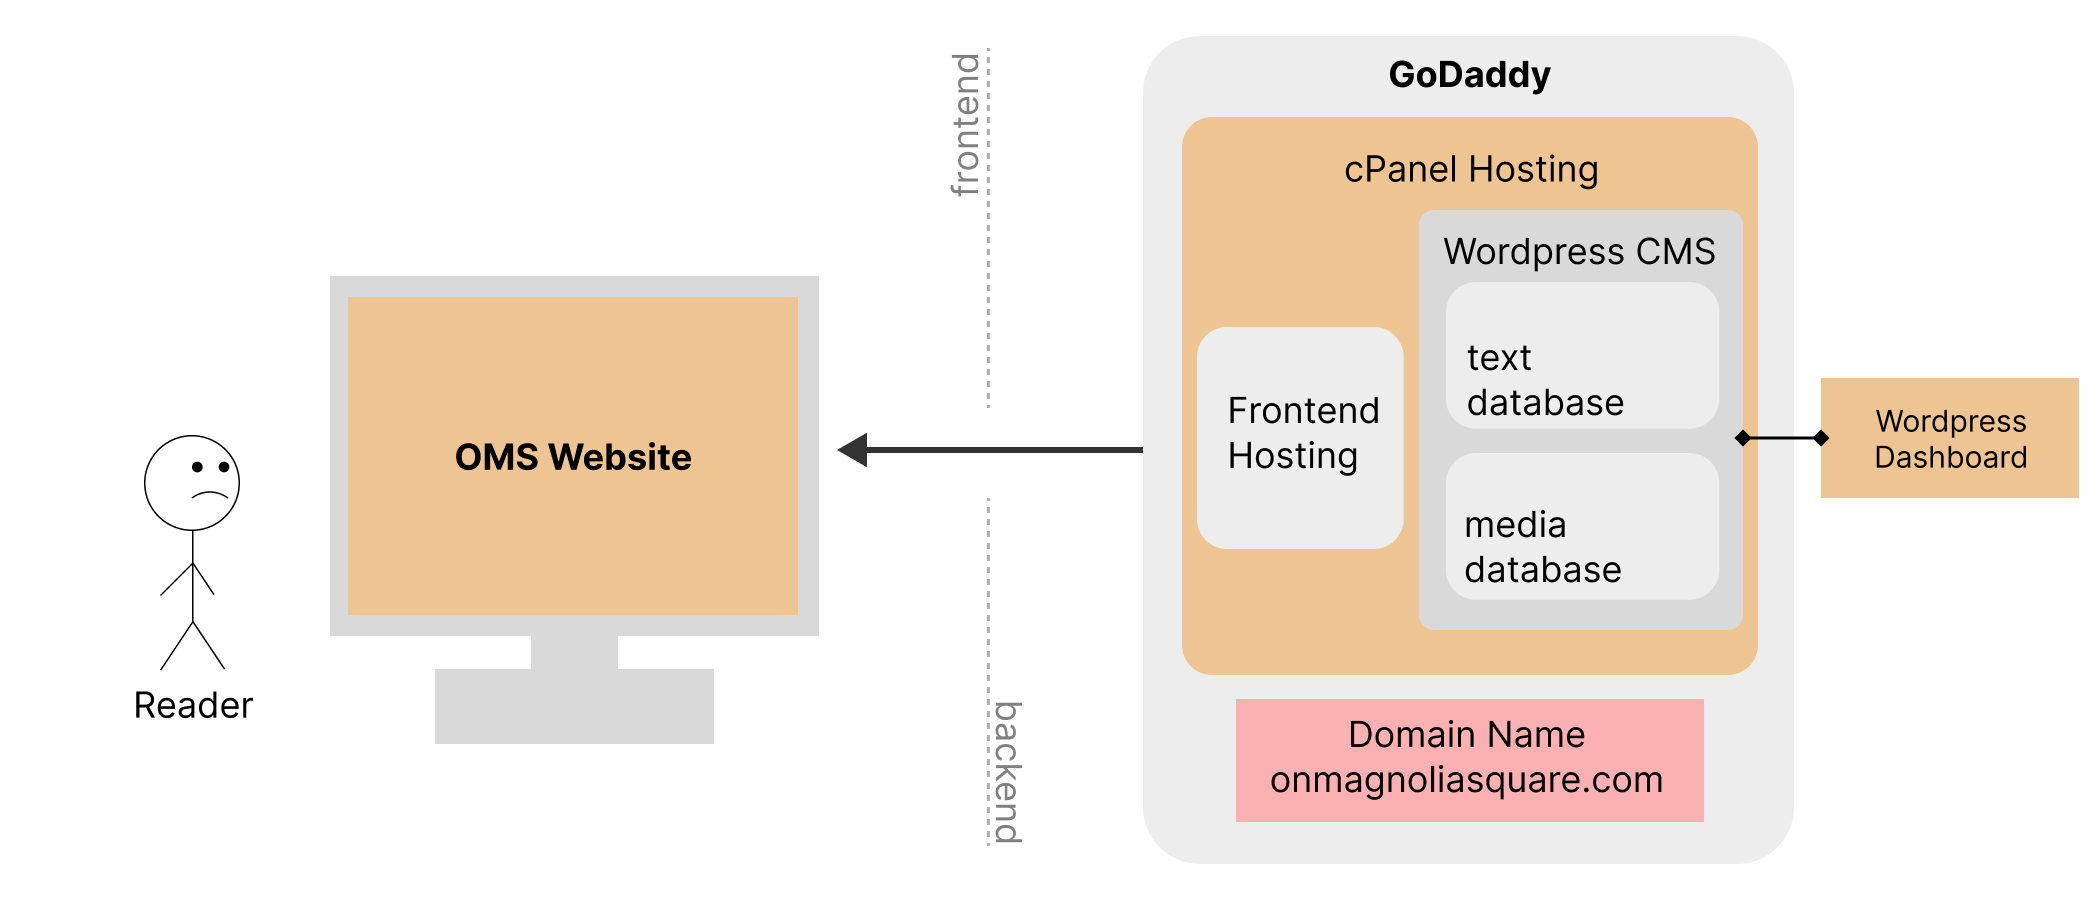
\includegraphics[scale=0.4]{diagrams/Frame 1.png}
    \caption{An End-To-End (E2E) infrastructure plan.}
    \label{fig:frame1}
\end{figure}

GoDaddy provides website hosting under \textit{cPanel}. cPanel hosts our Wordpress CMS, its accompanying text and media database, as well as the frontend. Content flows from the Wordpress dashboard, the place where publishers input text and images, into a text and media database, and then onto the frontend where readers can view the content.

\subsubsection{Issues}
Although all services are consolidated under one roof, this approach is prone to vendor lock-in and rigidity. In terms of §2.2, this system is somewhat accessible: the system operates on less surface area, which can be good since all services are in one place. However, it violates §2.2 Robustness and Future-proofing, because where it lacks in surface area it makes up in density. Density is how internally complicated and convoluted it can be to interface with the system in order to change, update, or improve it. I have personally explored the underbelly of GoDaddy's hosting dashboard and it is not pretty: the UI/UX can be confusing, sluggish, unintuitive, and prone to user error.

\subsection{Proposed Infrastructure}
My proposed infrastructure uses a Best-Of-Breed (BOB) solution. A BOB system is like composing a three-piece suit from materials sourced from the best silk and cotton mills; every component that constitutes the website is the crème de la crème, or for our purposes, the ones that suit our requirements the best.

\begin{figure}[h]
    \centering
    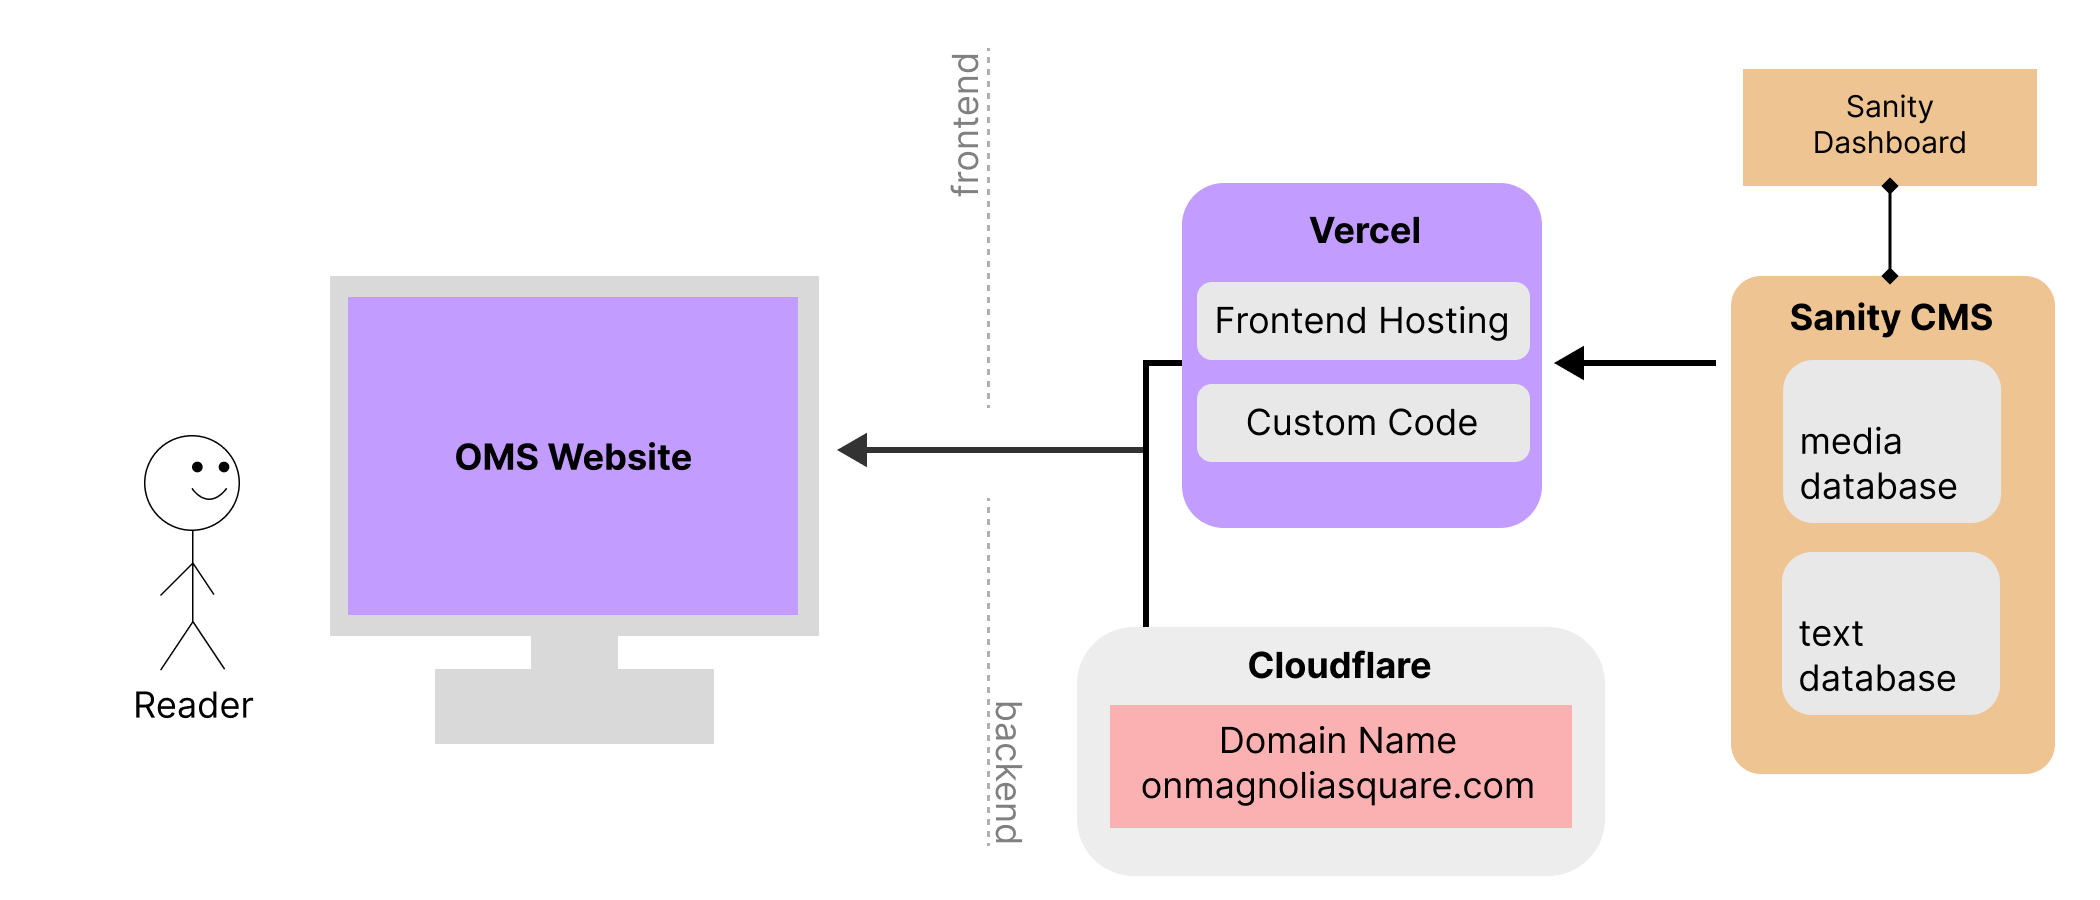
\includegraphics[scale=0.4]{diagrams/Frame 2.png}
    \caption{A Best-Of-Breed (BOB) infrastructure plan.}
    \label{fig:frame2}
\end{figure}

The flow of content follows a similar path to the GoDaddy E2E solution. It starts at a CMS dashboard, through to the CMS host, then to the frontend host, which is viewed by a reader when they access our domain name. The difference is the use of multiple services: Sanity is used as the CMS, Vercel is used as the frontend host, and Cloudflare is used as the domain name registrar.

Although BOB systems requires more surface area, the density of each service is manageable. For example, BOB systems are easier to debug and diagnose, because the components of the system are partitioned into discrete units with single responsibilities rather than consolidated into one box.

\subsubsection{Issues}
It requires some technical knowledge to know how these services interact with each other; some assembly is required. This means that there must be at least one OMS member technically oriented and also motivated to diagnose and fix an issue if it arises in the future. This may appear to violate §2.2 Future-proofing, because whoever joins the team may or may not be technically oriented, but the only hurdle to overcome this issue is knowledge and understanding. Anyone can execute it.

\subsection{Ditch or Fix?}
Distributing information online is always a sprinter's marathon: to achieve long term success, you must always be the quickest to adopt new tech. Therefore, rather than fixing the current infrastructure and ensuring that it maintains longevity into the future, I feel that it is better to ditch it, because the time spent attempting to fix and then ensuring the qualities of §2.2 are satiated is better spent on creating new infrastructure from the bottom up. Our small publication will require rocket engines strapped to its back to stay relevant. That cannot be done with our current infrastructure.
